\chapter{Methods}\label{chap:methods}
This chapter will describe the approaches used in order to go from the final problem statement, to a final product. The approaches are based on the knowledge acquired in \autoref{chap:analysis} and the design requirements found in \autoref{sec:DRequirements}.\\

While the product is being designed, two independent tests will be conducted. The first test will test usability during the design phase. This is to test whether the design is intuitive and the product is reliable.\\

The second test will test the validity of the final problem statement. This will create the basis of the conclusion chapter in the end of the report.\\

\section{Crawford slip}\label{sec:crawfordSlip}
In order to establish an initial design, the group will brainstorm and design different low fidelity prototypes, in order to establish pros and cons with different designs. 
The Crawford slip method is a process, where specific design criteria gets listed and combined, to figure out the main elements of the potential design\cite{crawfordSlip}.
of collecting single-sentence ideas on slips of paper, organizing the slips, analyzing, and then acting on them\cite{crawfordSlip}. The design made from the Crawford slip method, will be tested in an usability test.

\section{Usability test}

\subsection{Sampling}
The usability test will be conducted on the campus of Aalborg University for the sake of convenience. The students at Aalborg University can give valid feedback in terms of usability.\\

Therefore, the sampling technique used for the usability test is Convenience Sampling. Convenience sampling is a specific type of non-probability sampling method that relies on data collection from population members who are conveniently available to participate in a study. \cite{convSamp}\\
Convenience sampling is a type of sampling where the first available primary data source will be used for the research without additional requirements. In other words, this sampling method involves getting participants wherever you can find them and typically wherever is convenient.\cite{convSamp} In convenience, sampling no inclusion criteria identified prior to the selection of subjects. \cite{convSamp}\\

\section{System usability scale}\label{sus}
In order to gather concrete data from the usability test, the System Usability Scale(SUS)\cite{susScale} will be used. The SUS is a 10-item likert scale that is used to evaluate the usability of any given interactive system with both positively and negatively worded items. After the test is conducted, the participants select a number of the words, and combined they give a sense of the usability in the product\cite{susScale}.

\section{Target group test}

\subsection{Sampling}
In order to get feedback for the test to validate the final problem statement, it is necessary to conduct the test with the target group mentioned in \autoref{sec:targetgroup}. In order to get test participants that fit the needs of the target group and final problem statement, the quota sampling technique is used, as it bases the participants on pre-selected features or traits.\\

The Quota Sampling method is a sampling method that gathers representative data from a group.\cite{quotaSamp} As opposed to random sampling, quota sampling requires that representative individuals are chosen out of a specific subgroup\cite{quotaSamp}. For example, a researcher might ask for a sample of 100 females, or 100 individuals between the ages of 20-30\cite{quotaSamp}.

\subsection{Observation}\label{sec:observationalTest}
To get a better understanding of how the test group collaborates when using the prototype, and if they form some sort of group roles while using the prototype, a non-participant observational test was conducted\cite[p.~64-67]{bjoernerBog}. Using a non-participant test will prevent the observers from being a part of the test and potentially making the participants biased. Using this method of observation also symbolizes how the prototype would be used in a natural setting. A thing to keep in mind when conducting non-participant observations, is that the data relies heavily on the observers interpretation of the events. Therefore it is important that the observer knows exactly what to look for. In this test, the observers relied heavily on the information gained from the analysis about group roles and collaboration\cite[p.~64-67]{bjoernerBog}.\\\\

\section{Questionnaire and evaluation}
When the test have been conducted, the participants will answer a questionnaire. The questionnaire will be made as a Likert scale. This is to ensure that the data gathered from the test, can be analyzed and interpreted\cite{likertScale}.\\

By definition Likert scales are survey questions that offer a range of answer options — from one extreme attitude to another, like “extremely likely” to “not at all likely.” Typically, they include a moderate or neutral midpoint\cite{likertScale}.\\


Likert scales (named after their creator, American social scientist Rensis Likert) are quite popular because they are one of the most reliable ways to measure opinions, perceptions, and behaviors\cite{likertScale}.
Compared to binary questions, which give you only two answer options, Likert-type questions will get you more granular feedback about whether your product was just “good enough” or (hopefully) “excellent.” They can help decide whether a recent company outing left employees feeling “very satisfied,” “somewhat dissatisfied,” or maybe just neutral\cite{likertScale}.\\


This method will let you uncover degrees of opinion that could make a real difference in understanding the feedback you are getting. In addition, it can pinpoint the areas where you might want to improve your service or product\cite{likertScale}.\\

\subsection{Cronbach Alpha}\label{sec:cronbachAlpha}
To test validity of the questions in the Likert scale questionnaire, the Cronbach alpha method will be used \cite{DAEBook}. Cronbach alpha uses a mathematical formular, that tests the internal validity, that is measured as scale reliability. The test will output a value, that displays the validity of the questions\cite{DAEBook}.
\begin{figure}[H]
	\centering
	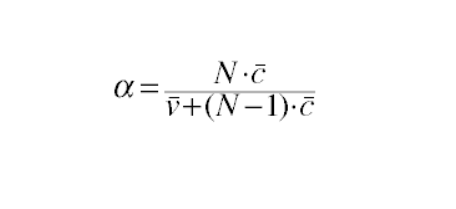
\includegraphics[width=0.9\linewidth]{figure/Methods/CAformel.png} 
	\caption{The formula used to calculate Cronbachs Alpha.}
	\label{fig:cronbachAlphaFormel}
\end{figure}
 


\subsection{Testing with children}
The test to validate the final problem statement will be conducted on the target group established in \autoref{sec:targetgroup} and is specified as children aged 8-12. The test to validate the final problem statement will be conducted on the target group. Therefore, it is necessary to establish a selection of elements that needs to be considered, when testing with children.\\

\textbf{Use age-appropriate language:} Don’t dumb it down, just simplify, especially when working across age groups\cite{testwithkids}.\\

\textbf{Be sensitive to maturity levels:} Specify grade levels or ages, instead of “teens,” specify age levels 13-15 and 16-19. Consider segmenting elementary school children, for example K-2nd or 3rd-5th, and adapting the test accordingly\cite{testwithkids}.\\

\textbf{Give yourself more time between sessions:} Working with younger children can take extra time and care and sessions can run over.\cite{testwithkids}\\

\textbf{Recruit more participants than you need:} This will help you in case there are absences or shy children\cite{testwithkids}.\\

\textbf{Recruiting:} Consider working with schools or other local facilities to recruit students. Most children are bound by their academic calendar, so working with schools enables you to test during the school day which provides you with greater options and faster turnaround for testing.  There’s the possibility of using school facilities—such as media equipment or wireless internet—which may simplify testing.  If you are able to get organizational buy in, it may encourage children to participate and parents to agree\cite{testwithkids}.\\

\textbf{Location:} Testing in a familiar environment, such as a school, library, or community facility will help your entire test run smoothly. A successful lab space for school aged children is a space that is familiar, convenient, and feels safe and secure\cite{testwithkids}.\\

Children are more aware than we give them credit for. Don’t try and hide the technology you’re using to capture the session; instead try to explain it and why you need it, e.g.
“There is a big magic mirror and my friends (client) are behind it. They’re going to watch what we do today and they’ll be talking to each other about how to fix things without disturbing you. We’ll go and say ‘Hi’ to them later on.”\cite{testwithkids}\\



